\section{System Design and Demo Walkthrough}
\label{sec:system}

\begin{figure*}[t]
\centering
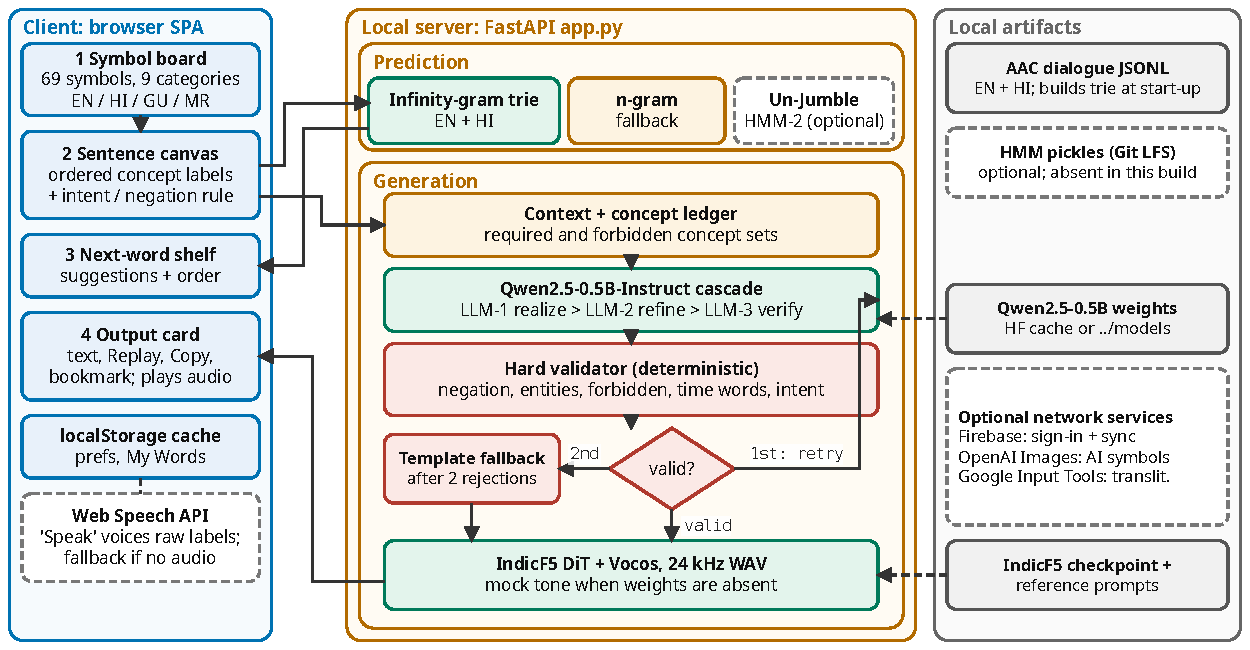
\includegraphics[width=\textwidth]{figures/architecture.pdf}
\caption{Architecture of the evaluated build. Solid boxes run locally; dashed boxes are optional or were absent (Git LFS HMM checkpoints, IndicF5 weights, network services). Between the columns, words flow to \texttt{/predict\_next}, the concept request to \texttt{/generate}, and text with \texttt{audio\_b64} back to the output card.}
\label{fig:arch}
\end{figure*}

\paragraph{Walkthrough.}
The user selects a language and taps symbols from a board of \NSymbols{} symbols in \NCategories{} categories, labeled in English, Hindi, Gujarati and Marathi (Figure~\ref{fig:ui}, \cn{1}); free text, an emoji search and a per-user ``My Words'' grid extend the vocabulary.
Selections accumulate on a sentence canvas (\cn{2}) while a shelf proposes next words (\cn{3}).
\emph{Speak} voices the literal labels with the browser's speech synthesis; \emph{AI Polish \& Speak} (\cn{4}) sends the selection to the local server and shows the returned sentence on an output card (\cn{5}) with Replay, Copy and bookmark controls.
The card is for review; the user revises a sentence by editing the canvas and regenerating.

\begin{figure*}[t]
\centering
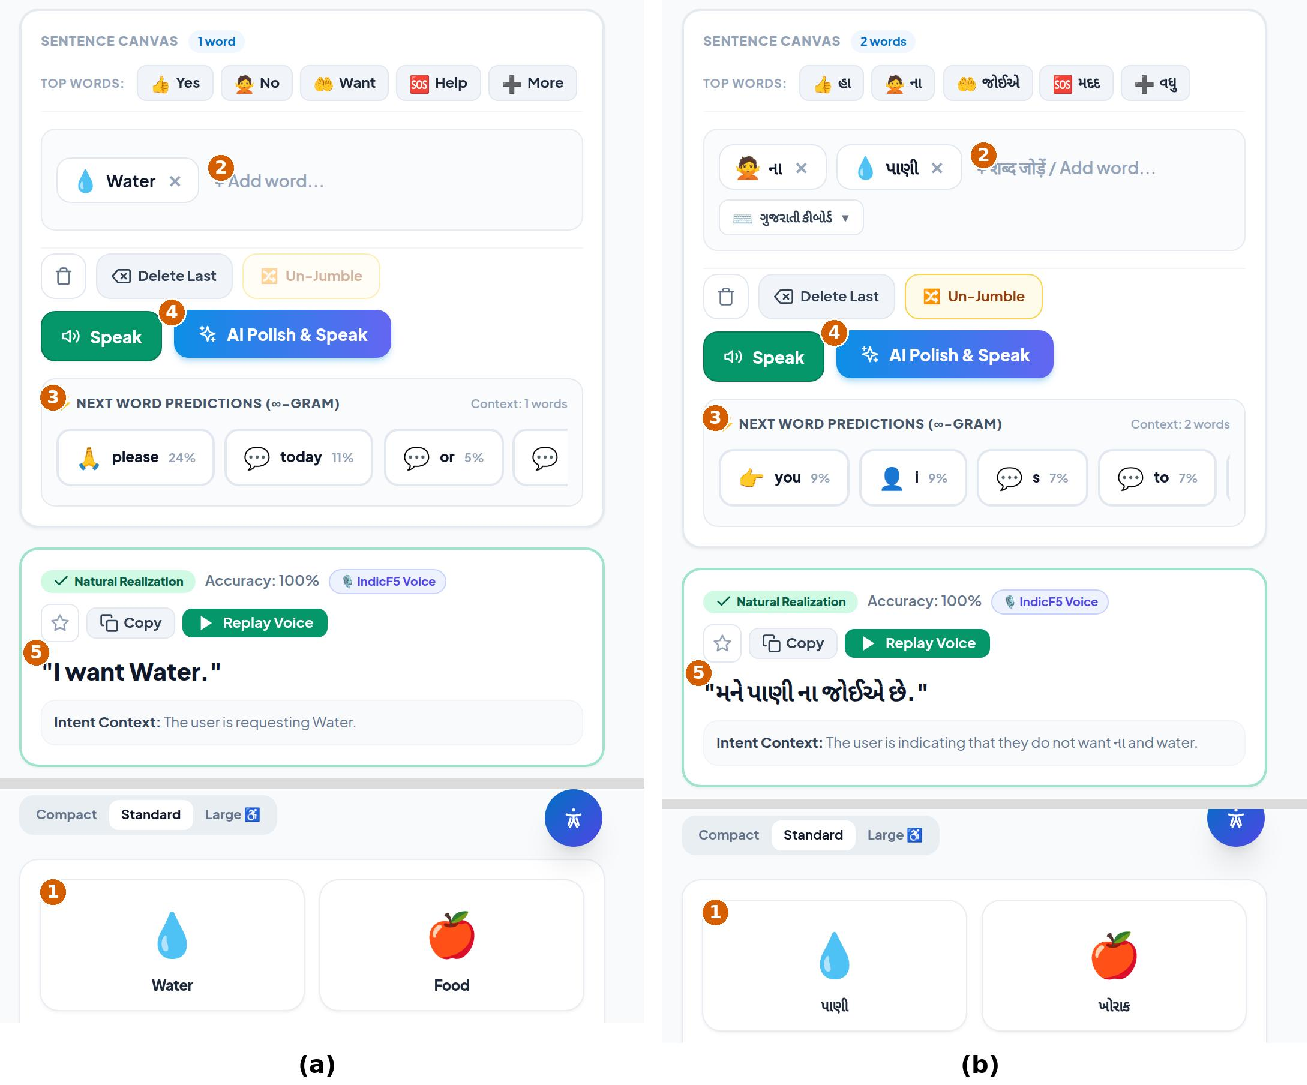
\includegraphics[width=0.74\textwidth]{figures/ui_panel.pdf}
\caption{Screenshots of the running build (Chrome, 520\,px viewport, signed-out default profile). (a)~English, \emph{Water}: the cascade output was rejected and the template returned. (b)~Gujarati, \gu{ના}+\gu{પાણી} (``no''+``water''): the cascade output was accepted; the shelf suggests English words (\S\ref{sec:eval}). Callouts: \cn{1} selected symbol, \cn{2} canvas, \cn{3} next-word shelf, \cn{4} generate, \cn{5} output sentence.}
\label{fig:ui}
\end{figure*}

\paragraph{Request and concept ledger.}
The client posts the ordered labels as \texttt{entities}, with \texttt{intent}, \texttt{negation}, \texttt{language}, \texttt{code\_mix}, \texttt{generation\_mode} and \texttt{voice\_id}, to \texttt{/generate}.
The web client infers \texttt{intent} and \texttt{negation} by substring rules over the labels (\textsc{negation} if a label contains \emph{no}, \emph{not} or a Hindi, Gujarati or Marathi negator; \textsc{question} for question words; \textsc{statement} for happy, sad, love and two Hindi labels; otherwise \textsc{request}); the API accepts the same fields from any client.
The server builds a \emph{ledger}: a required set (intent, actor, each selected entity, negation) and a forbidden set of 21 default words for unrequested times, meals and venues (e.g., \emph{tomorrow}, \emph{restaurant}), minus any word the user selected.

\paragraph{Realization and validation.}
Three prompted stages share one frozen Qwen2.5-0.5B-Instruct \citep{qwen2025qwen25}. LLM-1 realizes a sentence, from a few-shot prompt for Hindi, Gujarati and Marathi (12, 9 and 9 examples; greedy decoding) and from a ledger prompt for English and code-mixed output (temperature 0.1); LLM-2 removes unsupported content and is skipped for Indic-script candidates; LLM-3 returns a JSON verdict and a minimal rewrite.
A deterministic validator then decides. With $\nu$ the negation flag, $E$ the selected entities, $F$ the forbidden set and $y$ the candidate,
\begin{multline}
\mathrm{accept}(y)=[\mathrm{neg}(y)=\nu]\wedge\mathrm{match}(E,y)\\
\wedge\mathrm{intent}(y)\wedge\neg\mathrm{forbid}_F(y)\wedge\neg\mathrm{time}(y).
\label{eq:gate}
\end{multline}
Here \emph{neg} tests a fixed list of English, Hindi, Gujarati and Marathi negators; \emph{match} requires every selected entity to appear (a substring, plural and Indic-stem test); \emph{intent} rejects ``I want'' for feeling intents and requires a question cue for questions; \emph{forbid} matches words of $F$; and \emph{time} flags time words when none was selected.
A score in $[0,1]$ is displayed as \emph{Accuracy}, but the gate has no numeric threshold.
A rejection triggers one more cascade run; after two rejections a language-specific template built from the selected labels is returned (e.g., ``I want Water.'').
English and code-mixed attempts differ because LLM-1 samples; Indic attempts repeat because decoding is greedy.
The template is returned even if it fails the validator, and the card does not show that a fallback occurred.

\paragraph{Prediction and speech.}
Next-word suggestions come from an unbounded-order suffix-trie model with backoff 0.4, in the spirit of infini-gram \citep{liu2024infinigram}, built at start-up from the English and Hindi dialogue files (\IGSent{} sentences, \IGTok{} tokens); the trained HMMs serve as fallback and for \emph{Un-Jumble}.
Accepted text is synthesized by IndicF5 \citep{ai4bharat2025indicf5}, a flow-matching model of the F5-TTS family \citep{chen2025f5tts}, with a 24\,kHz Vocos vocoder \citep{siuzdak2023vocos}; a reference clip and its transcript condition the voice zero-shot.

\paragraph{Models and training.}
Table~\ref{tab:models} lists the learned components. The LLM and the speech model are used as released.
HMM-1 (interpolated 4-gram) and HMM-2 (word-and-POS trigram decoder) are trained by streaming external English text; the Hindi HMM and the infinity-gram model are trained on the AAC dialogues; an English flan-T5-small refiner is fine-tuned on template-generated payloads and reproduces at \RefAModelPct{} exact match on 384 group-disjoint payloads (Appendix~\ref{app:refiner}), but the server does not load it.

\begin{table*}[t]
\centering\footnotesize
\setlength{\tabcolsep}{3pt}
\begin{tabular}{@{}L{2.6cm}L{2.1cm}L{6.2cm}L{2.0cm}L{1.7cm}@{}}
\toprule
Component & Role & Training or adaptation & Data & In demo path \\
\midrule
Qwen2.5-0.5B-Instruct (rev.\ 7ae5576) & LLM-1/2/3 & None; prompted (few-shot for HI, GU, MR) & -- & yes \\
IndicF5 + Vocos & speech & Pretrained; zero-shot voice conditioning on a clip and transcript & 1,417\,h (4 corpora) & yes; weights not bundled \\
HMM-1, HMM-2 & next word; un-jumble & Streaming, 500K-sentence chunks (3 high-quality English, 2 Tatoeba, up to 500 Pile; log outside the artifact); pruning at counts 3 and 2. HMM-1: Jelinek--Mercer .50/.30/.15/.05. HMM-2: word and POS trigrams; exact search to 6 words, beam 64 above & external English text & yes, if checkpoints present \\
Gutenberg HMM & English bigram, trigram & 188,402 sentences; 63,783 bigram and 713,845 trigram states & public-domain books & legacy; Table~\ref{tab:pred} \\
Hindi AAC HMM & Hindi fallback & 3,867 turns of the Hindi dialogues; 2,171 word types & Hindi dialogues & fallback \\
Infinity-gram & next word (primary) & Count-based suffix trie built at start-up & EN, HI dialogues & yes \\
flan-T5-small refiner & English realization & Fine-tuned: 10 epochs (960 updates), learning rate $10^{-4}$, effective batch 32, seed 42 (Appendix~\ref{app:refiner}) & 3,052 template payloads & no \\
\bottomrule
\end{tabular}
\caption{Learned components. Sources: training scripts, run configurations and pickles in the artifact; the HMM-1 and HMM-2 checkpoints are Git LFS objects that were not available during evaluation. The four IndicF5 corpora are Rasa, IndicTTS, LIMMITS and IndicVoices-R.}
\label{tab:models}
\end{table*}
